\chapter{ПРАКТИЧНЕ ПОРІВНЯННЯ ТА РОЗШИРЕННЯ СИСТЕМИ}\label{ch:---:----}

У цьому розділі розглядаються практичні аспекти запропонованої симетричної криптосистеми на основі відображень кілець і систем лінійних рівнянь. Зокрема, наведено порівняння з поширеними симетричними та асиметричними алгоритмами, а також розглянуто потенціал використання протоколу у верифікованому шифруванні та протоколах з нульовим розголошенням. Для ілюстрації продуктивності використано результати тестування референсної (неоптимізованої) реалізації\footnote{Див. \url{https://github.com/KyrylR/sle-cryptosystem-wasm}}.

\section{Порівняння з подібними рішеннями}

\subsection{Загальні характеристики}

Запропонована система суттєво відрізняється від класичних симетричних (AES, ChaCha20) та асиметричних (ElGamal~\cite{elgamal}) криптосистем за такими критеріями:

\begin{table}[h!]
\centering
\begin{tabular}{|l|c|c|}
\hline
\textbf{Критерій} & \textbf{SLE} & \textbf{AES-256-GCM}~\cite{nist_gcm, rustcrypto_aes} \\
\hline
Тип & Симетрична & Симетрична \\
\hline
Структура ключа & Сукупність параметрів & 256-бітовий ключ \\
\hline
Налаштування & Складне, багатокрокове & Просте \\
\hline
Основа стійкості & Комбінаторика, алгебра & SPN, великий ключ \\
\hline
\end{tabular}
\caption{Порівняння основних характеристик}
\label{tab:table}
\end{table}

\begin{table}[h!]
\centering
\begin{tabular}{|l|c|c|}
\hline
\textbf{Критерій} & \textbf{SLE} & \textbf{ChaCha20Poly1305}~\cite{25, rustcrypto_chacha} \\
\hline
Випадковість & Вбудована & Через nonce \\
\hline
Розширення шифротексту & $\times 2$ & Мінімальне \\
\hline
Продуктивність & Помірна & Висока \\
\hline
\end{tabular}
\caption{Порівняння функціональних властивостей}
\label{tab:table2}
\end{table}

\textbf{Короткі висновки:}
\begin{itemize}
    \item SLE має складніший етап налаштування, але забезпечує великий простір ключів.
    \item Стандартні симетричні алгоритми (AES, ChaCha20) мають просту структуру ключа та надзвичайно високу швидкодію.
    \item SLE забезпечує ймовірнісне шифрування без додаткових режимів, але має розширення шифротексту.
\end{itemize}

\subsection{Порівняння швидкодії}

Нижче наведено результати тестування референсної реалізації SLE (неоптимізованої) у порівнянні з AES-256-GCM та ChaCha20Poly1305 для блоку даних розміром 1024 байти:

\begin{table}[h!]
\centering
\begin{tabular}{|l|c|c|c|}
\hline
\textbf{Алгоритм} & \textbf{SLE} & \textbf{AES-256-GCM}~\cite{nist_gcm, rustcrypto_aes} & \textbf{ChaCha20Poly1305}~\cite{25, rustcrypto_chacha} \\
\hline
Encrypt & 985~мкс & 7.25~мкс & 3.99~мкс \\
\hline
\end{tabular}
\caption{Час шифрування (1024 байти)}
\label{tab:table3}
\end{table}

\begin{table}[h!]
\centering
\begin{tabular}{|l|c|c|c|}
\hline
\textbf{Алгоритм} & \textbf{SLE} & \textbf{AES-256-GCM}~\cite{nist_gcm, rustcrypto_aes} & \textbf{ChaCha20Poly1305}~\cite{25, rustcrypto_chacha} \\
\hline
Decrypt & 306~мкс & 6.33~мкс & 3.50~мкс \\
\hline
\end{tabular}
\caption{Час дешифрування (1024 байти)}
\label{tab:table4}
\end{table}

\textbf{Висновки:}
\begin{itemize}
    \item SLE суттєво повільніший за сучасні симетричні алгоритми (на 2--3 порядки), що очікувано для прототипної реалізації на основі лінійної алгебри.
    \item Дешифрування у SLE швидше за шифрування, що пов'язано з особливостями протоколу.
    \item Наведені результати отримані для референсної (неоптимізованої) реалізації SLE\footnote{Див. \url{https://github.com/KyrylR/sle-cryptosystem-wasm}}; оптимізація може суттєво покращити продуктивність.
\end{itemize}

\section{Верифіковане шифрування та інтеграція з ZKP}
\label{sec:verifiable_encryption}

\textbf{Верифіковане шифрування} (verifiable encryption) --- це криптографічний підхід, який дозволяє довести правильність певної операції над зашифрованими даними (наприклад, правильність дешифрування, оновлення балансу, чи виконання обчислення) без розкриття секретного ключа чи самих даних.
Такий підхід є ключовим для побудови протоколів з нульовим розголошенням (Zero-Knowledge Proofs, ZKP~\cite{zkp_origin, pinocchio}), приватних транзакцій, а також для побудови довірених обчислень у розподілених системах, схематично представлений на рисунку~\ref{fig:zkp_interaction}.

\begin{figure}[ht]
    \centering
    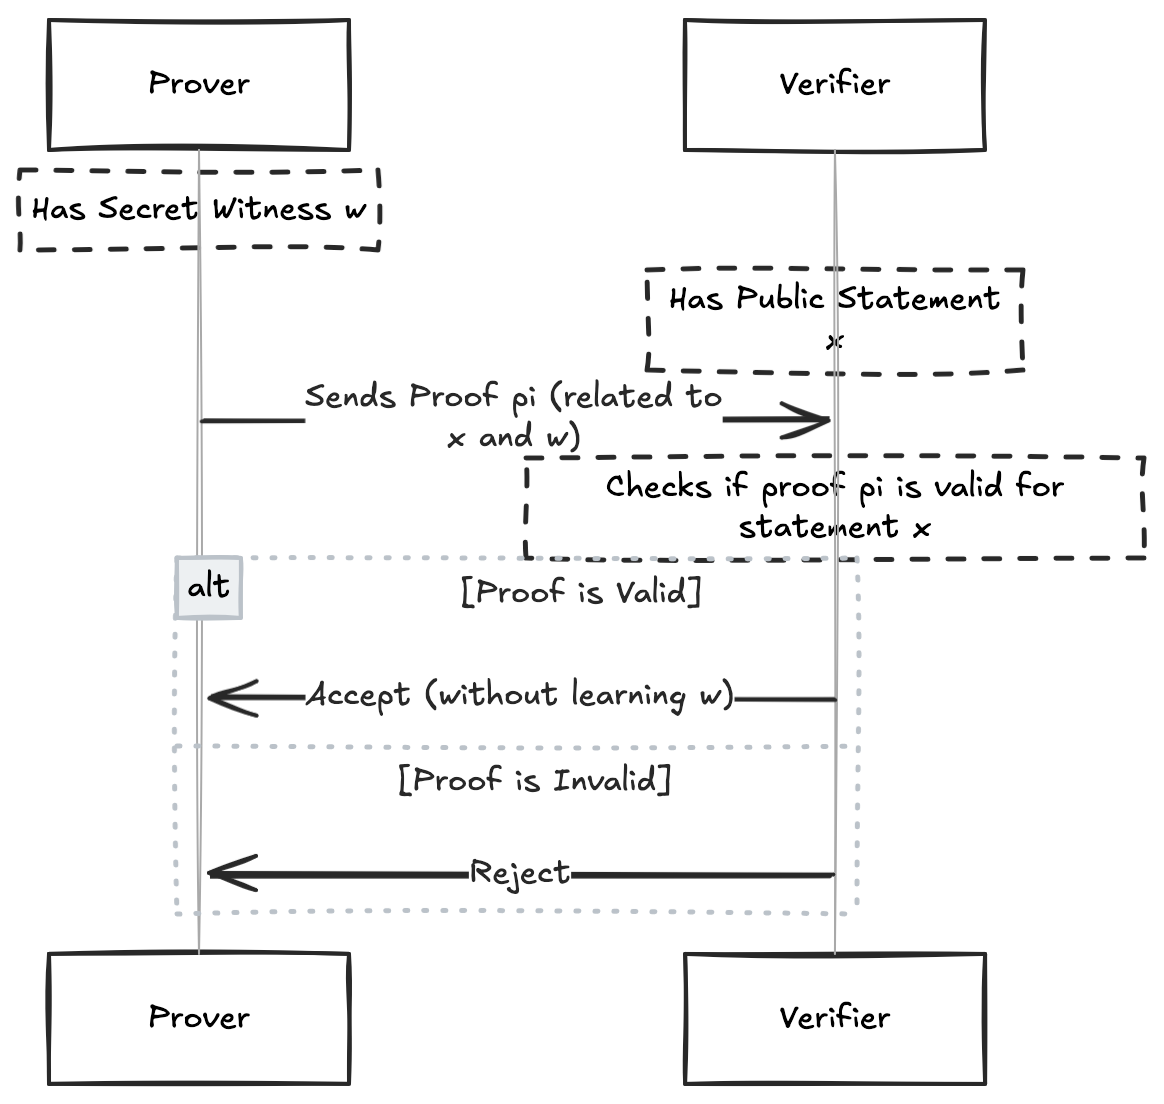
\includegraphics[width=0.4\textheight,keepaspectratio]{pictures/prover-verifier-image}
    \caption{Схематична взаємодія Prover та Verifier у протоколі з нульовим розголошенням.}
    \label{fig:zkp_interaction}
\end{figure}

\textbf{Мотивація:}
\begin{itemize}
    \item Забезпечення приватності: можна довести правильність обробки даних без їх розкриття.
    \item Протидія шахрайству: неможливо підробити доказ без знання секрету.
    \item Використання у блокчейнах, e-voting, приватних платіжних системах.
\end{itemize}

\subsection{SLE-протокол у контексті верифікованого шифрування}\label{subsec:sle-----}

SLE-протокол має алгебраїчну структуру (матричні та векторні операції, розв'язання СЛР), що робить його природним кандидатом для інтеграції з ZKP та верифікованим шифруванням.
Основна ідея полягає у тому, що всі операції протоколу можна виразити у вигляді арифметичних схем (R1CS~\cite{pinocchio}), які є стандартом для сучасних ZKP-систем (наприклад, zk-SNARK~\cite{14, 15}, zk-STARK~\cite{stark}).

Серед основних переваг SLE для верифікованого шифрування варто відзначити те, що всі операції протоколу базуються на лінійній алгебрі: робота з векторами та матрицями природно і компактно виражається у вигляді обмежень R1CS, що є стандартом для сучасних ZKP-систем.
Завдяки цьому, для малих розмірностей кількість модульних множень у SLE може бути значно меншою, ніж у схемах на основі піднесення до степеня (наприклад, ElGamal чи RSA), що знижує загальну складність доказу.
Крім того, структурованість лінійної алгебри дозволяє ефективніше оптимізувати схеми у ZKP-фреймворках.

Водночас існують і певні виклики.
По-перше, більшість сучасних ZKP-систем працюють над простими полями, тоді як SLE використовує арифметику у кільці, і емуляція такої арифметики за складеним модулем $m$ може бути обчислювально затратною.
По-друге, якщо відображення у протоколі визначаються великими таблицями, їх ефективне представлення у R1CS є складним; ситуація спрощується лише у випадку, коли відображення мають явну арифметичну формулу.
Нарешті, для складних операцій, таких як обернення матриці, розмір відповідної схеми R1CS може суттєво зрости, що впливає на швидкість генерації та перевірки доказу.

\subsection{Порівняння SLE та ElGamal у контексті ZKP}\label{subsec:-sle--elgamal---zkp}

Типові сценарії застосування верифікованого шифрування включають доведення коректного дешифрування, коли необхідно переконати сторонню особу, що зашифроване повідомлення було правильно розшифроване без розкриття секретного ключа.
Іншим поширеним випадком є доказ оновлення балансу: потрібно підтвердити, що новий шифротекст дійсно відповідає оновленому балансу, не розкриваючи саму суму.
Нарешті, важливим застосуванням є доказ коректного виконання обчислення, коли необхідно довести, що над зашифрованими даними була виконана дозволена операція згідно з протоколом, не розкриваючи вхідні чи проміжні значення.

\textbf{Загальна схема інтеграції SLE з ZKP:}
\begin{enumerate}
    \item Формалізувати операцію (наприклад, дешифрування) як арифметичну схему.
    \item Виразити її у вигляді R1CS (Rank-1 Constraint System~\cite{pinocchio}).
    \item Згенерувати доказ (наприклад, zk-SNARK~\cite{14, 15}) для цієї схеми.
    \item Передати доказ разом із шифротекстом для перевірки.
\end{enumerate}

У схемах на основі піднесення до степеня (ElGamal~\cite{elgamal, 12}) доведення коректності операцій у ZKP є дорогим через велику кількість мультиплікативних обмежень.
У SLE основні операції — це додавання та множення у кільці, що може бути значно ефективніше для ZKP, особливо для невеликих розмірностей.

SLE-протокол може бути перспективним для застосувань, де потрібне верифіковане шифрування або інтеграція з ZKP, особливо якщо вдасться ефективно реалізувати арифметику у кільці та відображення у сучасних ZKP-фреймворках.
Однак практична ефективність залежить від конкретної реалізації та обмежень обраної ZKP-системи.
